\section{Design}
\label{sec:design}

Houdini is built using Python 3 and leverages a QEMU KVM VM to provide a controlled testing environment for container security validation. Instead of running containers directly on the host system, Houdini spins up a dedicated VM, ensuring that any security tests remain isolated and do not affect the host system.

At the core of Houdini’s architecture, a Flask-based server runs on the host operating system. This server acts as a bridge between the host and the QEMU KVM VM, facilitating communication between them. The Flask server is responsible for sending commands and configuration data to the guest VM and receiving trick execution results. When a trick is initiated, the Houdini client on the host instructs the VM to start a new trick. The VM then launches a container with the specified security configurations and executes the trick inside it.  

Once the trick completes, the VM collects the results and sends them back to the host via the Flask server. The host then processes this data, logs the results, and determines whether the trick passed. A trick in Houdini is a structured security check designed to evaluate whether a containerized environment enforces confinement properly. Each test systematically probes specific security controls (e.g., namespaces, cgroups, capabilities) to determine if a container remains within its intended isolation boundaries or if a misconfiguration, vulnerability, or unexpected behavior allows for unintended behaviour such as, but not limited to privilege escalation, resource leakage, or escape.

 This structured workflow ensures that Houdini remains independent of the host system’s container runtime while providing a reliable and repeatable environment for testing container confinement mechanisms.

\begin{figure}[h]
  \label{fig:state-machine}
  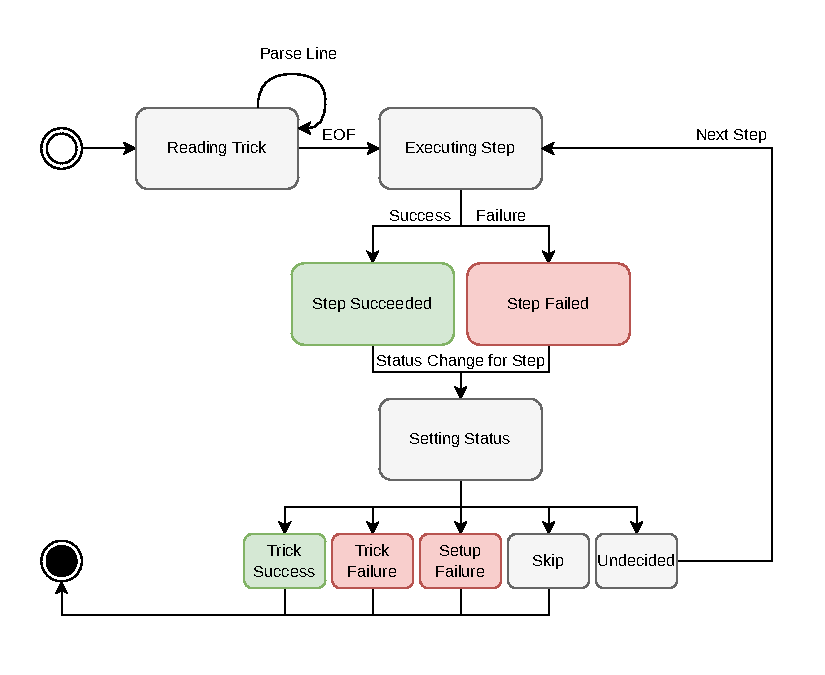
\includegraphics[width=1\linewidth]{figs/houdini-state-machine.pdf}
  \caption{A state machine diagram of Houdini running a Trick.}
\end{figure}
